\section{Движение тела под углом к горизонту}

\begin{ex} 
Камень брошен с высоты $h$ под углом $\alpha$ к горизонту  со скоростью $v_0$. Какой угол $\beta$ будет составлять скоростью камня с горизонтом в момент падения на землю? Чему равна величина этой скорости? На каком расстоянии $s$ по горизонтали от основания точки запуска упадет камень?
\begin{ans}
$\tan \beta = \sqrt{\tan^2 \alpha + \frac{2gh}{v_0^2 \cos^2 \alpha}}$, $s=\frac{v_0 \cos \alpha}{g} \sqrt{v_0^2 \sin^2 \alpha + 2gh}$.
\end{ans}
\end{ex}

\begin{ex}
Мальчик бросает камень по направлению в кота, сидящего на крае сарая. Через 1 секунду камень падает на землю в точку, находящуюся на одной вертикали с котом. На какой высоте находился кот?
\begin{ans}
$h = g\tau^2/2 = 5$ м		
\end{ans}
\end{ex}	

\begin{ex} 
Мышонок стреляет из рогатки в кота, сидящего на ветке дерева. Через $t = 1$ с камень попадает в ветку прямо у лап кота. На каком расстоянии $s$ от мышонка находился кот, если известно, что векторы $\vec v(0)$ и $\vec v(t)$ взаимно перпендикулярны? 
Ускорение свободного падения $g$ = 10 м/с\textsuperscript{2}. Сопротивление воздуха пренебрежимо мало.
\begin{ans}
$h = gt^2/2 = 5$ м
\end{ans}
\end{ex}

\begin{ex}
Камень бросили с горизонтальной площадки под углом к горизонту в направлении вертикальной стены. Камень упруго ударился о стену и упал на площадку. Известно, что время полёта от момента бросания до удара составило $t_1$, а время полёта от удара до падения $t_2$. Определите, на какой высоте камень ударился о стену. Стена перпендикулярна плоскости, в которой движется камень. Влиянием воздуха можно пренебречь.
\begin{ans}
$h = gt_1t_2/2$
\end{ans}
\end{ex}

\begin{ex}
Маленький шарик, брошенный с начальной скоростью $\vec{v}_0$ под углом $\alpha$ к горизонту, 
ударился о вертикальную стенку, движущуюся ему навстречу с горизонтально направленной скоростью $\vec u$, и отскочил в точку, из которой был брошен. 
Определите, через какое время $t_1$ после броска произошло столкновение шарика со стенкой? Потерями на трение пренебречь.
\begin{sol}
Пусть время движения от соударения до возвращения в точку бросания равно $t_2$. Поскольку при упругом ударе вертикальная составляющая скорости не меняется, а горизонтальная скорость увеличивается до величины $v_0 \cos \alpha + 2u$, то полное время полета составит $t_1 + t_2 = \frac{2v_0 \sin \alpha}{g}$. Расстояние по горизонтали от места броска до места удара о стенку выражается в виде $v_0 \cos \alpha t_1 = (v_0 \cos \alpha +2u)t_2$, откуда $t_1 = \frac{v_0 \sin \alpha (v_0 \cos \alpha + 2u)}{g(v_0 \cos \alpha + u)}$.
\end{sol}
\begin{ans}
$t_1 = \frac{v_0 \sin \alpha (v_0 \cos \alpha + 2u)}{g(v_0 \cos \alpha + u)}$
\end{ans}
\end{ex}

\begin{ex}
С какой минимальной скоростью можно перебросить камень через здание высоты $H$ с куполообразной крышей радиуса $R$?
\begin{ans}
$v_{min} = \sqrt{g(R+2H)}$
\end{ans}
\end{ex}

\begin{ex}
Зенитное орудие может сообщить снаряду начальную скорость $v_0$ в любом направлении. Требуется найти зону поражения, т.е. границу отделяющую цели, до которых снаряд из данного орудия может долететь, от недостижимых целей. Сопротивлением воздуха пренебречь. 
\begin{ans}
$y = \frac{v_0^2}{2g} - \frac{gx^2}{2v_0^2}$
\end{ans}
\end{ex}

\begin{ex}
В спортивном зале высотой $h$ бросают маленький мяч с начальной скоростью $v_0$. Определите, какое максимальное расстояние по горизонтали может пролететь мяч после бросания до первого удара о пол, если соударение с потолком абсолютно упругое. Считайте, что мяч бросают с уровня пола. Пол и потолок горизонтальны, сопротивление воздуха пренебрежимо мало.
\begin{ans}
Если $v_0 < 2 \sqrt{gh}$, то дальность полета $L = \frac{v_0^2}{g}$; если $v_0 > 2 \sqrt{gh}$, то $L = 4h \sqrt{\frac{v_0^2}{2gh}-1}$.
\end{ans}
\end{ex}

\begin{ex}
Необходимо с поверхности земли попасть камнем в цель, расположенную на расстоянии $L$ по горизонтали на высоте $H$. С какой наименьшей скоростью это можно сделать? Трением пренебречь.
\begin{ans}
$v_{min} = \sqrt{g \left(\sqrt{l^2 + h^2} + h \right)}$
\end{ans}
\end{ex}

\begin{ex}
(2004) При какой минимальной начальной скорости $v_0$ можно перебросить камень через дом с покатой крышей? 
Ближайшая стена имеет высоту $H$, задняя стена -- высоту $h$, ширина дома равна $l$.
\begin{center}
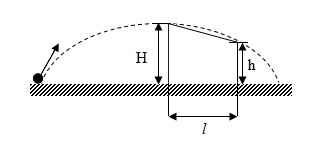
\includegraphics[width=5.0cm]{0209AngleHouse.jpg}
\end{center}
\begin{sol}
Требование минимальности скорости бросания камня с поверхности земли означает, что оптимальная траектория камня пройдет через точки "вершины" крыши В и С, расположенные на высотах $H$ и $h$ соответственно. Обратим движение камня и определим минимальную скорость в точке C -- $v_C$, при которой камень может перелететь через точку В. Учитывая решение предыдущей задачи, легко понять, что $v_B = \sqrt{g \left(\sqrt{l^2 + (H-h)^2} + H-h \right)}$. Минимально возможную скорость бросания камня с земли $v_{min}$ найдем из закона сохранения энергии $v_{min}^2 = v_B^2 + 2gH$, откуда $v_{min} = \sqrt{g \left(\sqrt{l^2 + (H-h)^2} + H + h \right)}$.
\end{sol}
\begin{ans}
$v_{min} = \sqrt{g \left(\sqrt{l^2 + (H-h)^2} + H + h \right)}$
\end{ans}
\end{ex}

\begin{ex}
(2018) Тело бросают с поверхности длинной наклонной плоскости. Угол наклона плоскости к горизонту $\alpha = 45^{\circ}$, величина начальной скорости фиксирована. 1) Под каким углом к горизонту нужно бросить тело для того, чтобы время полета было максимально? 2) Под каким углом к горизонту нужно бросить тело для достижения максимальной дальности (дальность откладывается вдоль плоскости)?
\begin{ans}
1) $\pi/2$; 2) $\pi/8$
\end{ans}
\end{ex}

\begin{ex}
(2005) Колесо радиуса $R$ катится по горизонтальной мокрой дороге со скоростью $v$. 1) На какую максимальную высоту $h$ поднимаются капли воды, отрывающиеся от колеса? 2) Какой должна быть минимальная скорость колеса, чтобы капелька, достигшая максимальной высоты, опустилась на то же самое место? 3) Изменится ли высота $h$, если колесо будет катиться с пробуксовкой?
\begin{ans}
1) При $gR > v^2$ максимальная высота подъема $h = 2R$, при $gR < v^2$ -- $h = R +\frac{v^2}{2g} + \frac{gR^2}{2v^2}$; 2) $v_{min} = \frac{\pi g R}{(1+ \sin \alpha) \cos \alpha}$, где $\sin \alpha = gR/v^2$; 3) изменится.
\end{ans}
\end{ex}

\begin{ex}
(2010) В сферической лунке прыгает шарик, упруго отражаясь от ее стенки в двух точках, расположенных на одной горизонтали. Промежуток времени при движении шарика слева направо равен $T_{1}$, а при движении справа налево -- $T_2$. Определите радиус лунки.
\begin{ans}
$R = \sqrt{g} T_1 T_2 /2\sqrt{2}$
\end{ans}
\end{ex}

\begin{ex}
Из точек A и В, находящихся на одной горизонтальной прямой, одновременно бросили два камня с одинаковыми по модулю скоростями $v_0$ = 20 м/с. 
Один из камней полетел по навесной траектории, другой -- по настильной, но каждый попал в точку старта другого камня. 
Известно, что в точке А угол бросания $\alpha = 75^{\circ}$. 
Через какое время $\tau$ после старта расстояние между камнями станет минимальным? Чему равно это расстояние?
\begin{ans}
$s = 10$ м, $\tau = v_0 \sin 150^{\circ} \cos 30^{\circ} \cos 45^{\circ} /g$
\end{ans}
\end{ex}

\begin{ex}
Две частицы одновременно начали двигаться в однородном поле тяжести $\vec g$. Начальные их скорости равны по модулю $v_0$ и лежат в одной вертикальной плоскости. Угол наклона вектора одной из скоростей к горизонту равен $\alpha$, а другой $2\alpha$. В какой момент времени $\tau$ от начала движения скорости частиц окажутся сонаправленными? Сопротивлением движению пренебречь.
\begin{ans}
$\tau = \frac{v_0 \cos (\alpha /2)}{g \sin (3\alpha / 2)}$
\end{ans}
\end{ex}

\begin{ex}
Шарик, которому сообщена горизонтальная скорость $v$, падает на горизонтальную плиту с высоты $h$. При каждом ударе о плиту вертикальная составляющая скорости уменьшается (отношение вертикальной составляющей скорости после удара к ее значению до удара постоянно и равно $\alpha$). Определить, на каком расстоянии $х$ от места бросания отскоки шарика прекратятся. Считать, что трение отсутствует, так что горизонтальная составляющая скорости шарика $v$ не меняется.
\begin{ans}
$x = v \sqrt{2h/g} \left( 1 + \alpha \right) / \left( 1 - \alpha \right)$
\end{ans}
\end{ex}